\section{Background and Problem Setup}\label{background}
This section describes the challenges in predictive modeling after progressive data 
cleaning and describes concrete example applications.

\subsection{Dirty Data Model}\label{dmodel}
This paper explores a model for data error where attributes of records in a relation $R$ are incorrect or missing.
Formally, there exists a record-by-record cleaning operation $C(\cdot)$ can be applied to a record $r \in R$ to recover $r_{clean}$.
The information in a record $r$ is sufficient to uniquely determine $r_{clean}$. 
%Following from this model, there are two relations $R_{dirty}$ and $R_{clean}$ with the same schema and a one-to-one mapping between rows.
Therefore, for every $r \in R_{dirty}$ there exists an $r' \in R_{clean}$, and a cleaning function $C(\cdot)$, is a function that maps each $r$ to its corresponding $r'$.
We assume that there is a featurization $F(\cdot)$ which is defined over both $R_{dirty}$ and $R_{clean}$ and maps rows to vectors in $\mathbb{R}^d$.
So each row corresponds to one training example in the predictive model.

A number of common data cleaning techniques can be modeled in this way.
For example, fixing attributes with inconsistent representations, updating out-of-date data, imputing missing attribute values, and enforcing record-level data quality constraints.
On the other hand, there a number of techniques that cannot be posed as a row-by-row mapping such as deduplication and schema matching.

\subsection{Active Learning and Data Cleaning}
There are a number of recent approaches that apply active learning to reduce number of records that need to be cleaned by a human.
The main idea is to treat human input as binary labels in a supervised learning problem \cite{DBLP:journals/pvldb/MozafariSFJM14}.
For example, Gokhale et al. \cite{gokhale2014corleone} applies crowdsourcing to label likely pairs of records as duplicates.
Yakout et al. \cite{DBLP:journals/pvldb/YakoutENOI11} proposed a technique called Guided Data Repair, where human input was used to confirm proposed repairs that satisfy pre-declared data quality rules.
In Gokhale et al. and Yakout et al., the goal of the learning model is to anticipate the human input and only require labels when uncertain.

Active learning is a very powerful and general concept that goes beyond binary labels and essentially argues that not all information is created equal.
It iteratively uses the current best model to acquire the most valuable future data.
We explore how to apply this idea to analysis-driven data cleaning. 
Some data are more relevant than others to a downstream analytics, and thus, more valuable to clean.
However, the problem of prioritzing cleaning by using a user-specified downstream model is subtly different than active learning as currently applied in data cleaning.
Using machine learning to enhance data cleaning means predicting clean data from dirty data.
In \sys, machine learning is the data analysis and this requires predicting clean data from \emph{clean data}.
This small change raises a number of challenges in ensuring correctness and priotization.

It turns out that these two definitions are not incompatible and \sys explores a more general problem setting.
For example, rather than replacing the dirty data, corresponding clean data can be added into new columns. 
Thus, \sys can be used to train models for some learning-based data cleaning algorithms.
It can apply in a wider set of problems than existing work such as when data quality rules do not exist and numerical value imputation where human input is not binary.

\subsection{Correctness}  
The key challenge in \sys is correctness of the statistical model.
The straight-forward application of progressive or incremental data cleaning methods proposed in the literature is to fix those errors in place.
Suppose $k \ll N$ records are cleaned, but all of the remaining dirty records are retained in the dataset.
Figure \ref{update-arch1} highlights the dangers of this approach on a very simple dirty dataset and a linear regression model i.e., the best fit line for two variables. 
One of the variables is systematically corrupted with a translation in the x-axis (Figure \ref{update-arch1}a).
The dirty data is marked in brown and the clean data in green, and their respective best fit lines are in blue.
After cleaning only two of the data points (Figure \ref{update-arch1}b), the resulting best fit line is in the opposite direction of the true model.
This is a well-known phenomenon called Simpsons paradox, where mixtures of different populations of data can result in spurious relationships \cite{simpson1951interpretation}.
Training models on a mixture of dirty and clean data can lead to unreliable results, where artificial trends introduced by the mixture can be confused for the effects of data cleaning.

\begin{figure}[ht!]
\centering
 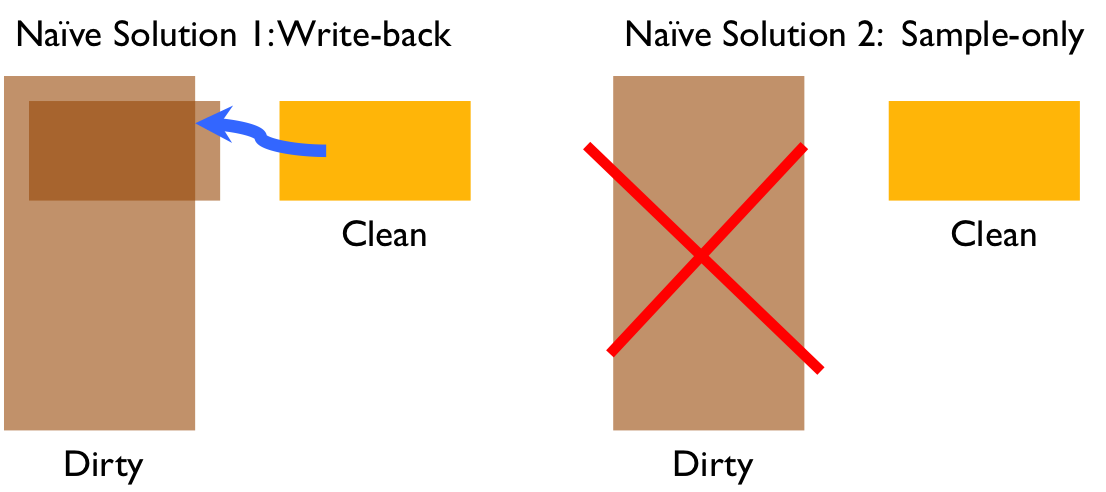
\includegraphics[width=\columnwidth]{figs/update-arch.png}
 \caption{(a) Systematic corruption in one variable can lead to a shifted model. 
 (b) Mixed dirty and clean data results in a less accurate model than no cleaning.
(c) Small samples of only clean data can result in similarly inaccurate models. \label{update-arch1}}
\end{figure}

An alternative is to avoid the dirty data altogether instead of mixing the two populations.
Suppose $k$ records are randomly sampled from the dataset and cleaned.
The model is trained only on the cleaned sample of data.
This is similar to SampleClean \cite{wang1999sample}, which was proposed to approximate the results of aggregate queries by applying them to a clean sample of data.
However, high-dimensional models are highly sensitive to sample size.
Figure \ref{update-arch1}c illustrates that, even in two dimensions, models trained from small samples can be as incorrect as the mixing solution described before.

\subsection{Intuitive Solution}
Our first goal is to find an update methodology that avoids Simpson's Paradox and the strong dependence on sample size.
Instead of mixing dirty and clean data, \sys uses a model trained on the dirty data as an initialization, and then iteratively updates this model using samples of clean data.
The intuition is that this algorithm smoothly transitions the model from one population (the dirty data) to another (the clean data), leading to provable guarantees about intermediate results.
Our next goal is to priotize which data to clean based on information from the model.
We design \sys to make greater progress at these small sample sizes using the dirty model as an initialization.
Doing so is not trivial since data may look unimportant to a dirty model but when cleaned are very important.
Also, data cleaning and model training can happen at very different time scales, we have to carefully budget our effort to ensure that any optimizations actually address rate-determining steps in the workflow.

\subsection{Use Case: Dollars for Docs \cite{dollarsfordocs}}
ProPublica collected a dataset of corporate donations to doctors to analyze conflicts of interest. 
They reported that some doctors received over \$500,000 in travel, meals, and consultation expenses \cite{dollarsfordocsa}.
ProPublica laboriously curated and cleaned a dataset from the Centers for Medicare and Medicaid Services that listed nearly 250,000 research donations, and aggregated these donations by physician, drug, and pharmaceutical company.
We collected the raw unaggregated data and explored whether suspect donations could be predicted with a model.
This problem is typical of analysis scenarios based on observational data seen in finance, insurance, medicine, and investigative journalism.
The dataset has the following schema:
\begin{lstlisting}[mathescape,basicstyle={\scriptsize}]
Contribution(pi_specialty$\textrm{,}$ drug_name$\textrm{,}$ device_name$\textrm{,}$
corporation$\textrm{,}$ amount$\textrm{,}$ dispute$\textrm{,}$ status)
\end{lstlisting}

\noindent\texttt{pi\_specialty} is a textual attribute describing the specialty of the doctor receiving the donation.

\noindent\texttt{drug\_name} is the branded name of the drug in the research study (null if not a drug).

\noindent\texttt{device\_name} is the branded name of the device in the study (null if not a device).

\noindent\texttt{corporation} is the name of the pharmaceutical providing the donation.

\noindent\texttt{amount} is a numerical attribute representing the donation amount.

\noindent\texttt{dispute} is a Boolean attribute describing whether the research was disputed.

\noindent\texttt{status} is a string label describing whether the  donation was allowed under the declared research protocol. The goal is to predict disallowed  donation. 

\vspace{0.5em}

However, this dataset is very dirty, and the systematic nature of the data corruption can result in an inaccurate model.
On the ProPublica website \cite{dollarsfordocs}, they list numerous types of data problems that had to be cleaned before publishing the data (see Appendix \ref{dfd-errors}).
For example, the most significant donations were made by large companies whose names were also more often inconsistently represented in the data e.g., ``Pfizer Inc.", ``Pfizer Incorporated", ``Pfizer".
In a scenario such as this one, the effect of systematic error can be serious.
Duplicate representations could artificially reduce the correlation between these entities and suspected contributions.
There were nearly 40,000 of the 250,000 records that had either naming inconsistencies or other inconsistencies in labeling the allowed or disallowed \texttt{status}.
Without data cleaning and using a Support Vector Machine model, the detection rate of suspect donations was 66\%.
Applying the data cleaning to the entire dataset improved this rate to 97\% in the clean data (Section \ref{dfd-exp}), and the experiments describe how \sys can achieve an 80\% detection rate for less than 4000 records cleaned.


%\sys avoids both pitfalls, Simpson's paradox and sample size dependence.

\iffalse
\sys avoids both pitfalls, Simpson's paradox and sample size dependence.
In Section \ref{model-update}, we show how we do this with iterative gradient steps (i.e., incrementally moving the line based on the clean data).
This takes advantage of the dirty data as well as the clean data, but still have provable properties about the intermediate results.
The intuition is that it smoothly and iteratively transitions the model from one population (the dirty data) to another (the clean data).
In Figure \ref{sys-arch2}, we illustrate our ideal tradeoff space of sampling and data cleaning.
At two extremes we have no cleaning (just using the dirty data) and full cleaning.
%\sys is optimized for convergence for smaller sample sizes than a uniform sampling approach.

\begin{figure}[t]
\centering
 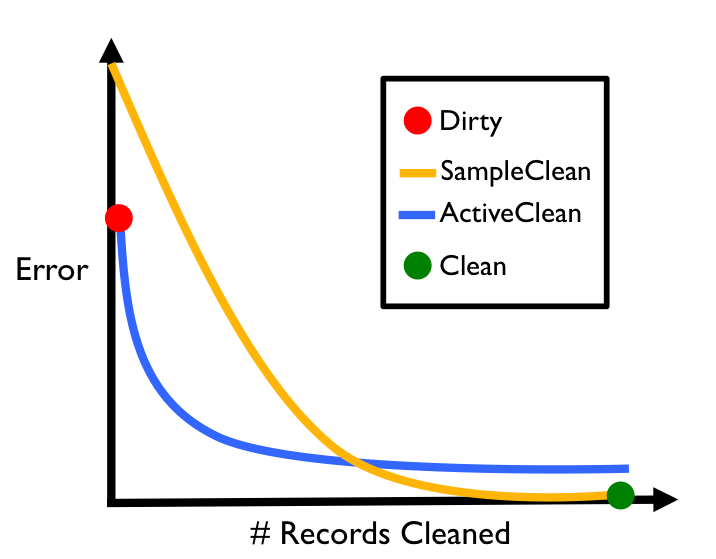
\includegraphics[width=0.5\columnwidth]{figs/arch2.png}
 \caption{\sys is designed to converge to an accurate model with fewer cleaned records than a uniform sampling approach (SampleClean). \label{sys-arch2}}\vspace{-1em}
\end{figure}


We design \sys to make greater progress at these small sample sizes using the dirty model as an initialization.
Doing so is not trivial since it requires analysis of both the Machine Learning model and the data cleaning operations.
Data may look unimportant to a dirty model but when cleaned are very important.
Also, data cleaning and model training can happen at very different time scales, we have to carefully budget our effort to ensure that any optimizations actually address rate-determining steps in the workflow.
Finally, in this line of work, the tradeoff space is enormous, and we have to carefully pick a design point and tailor our optimizations to this preferred regime.
\fi

%Consider the data corruption in our motivating example where company names were inconsistently entered: ``Pfizer Inc.", ``Pfizer Incorporated", ``Pfizer".
%Fixing this error can be represented as a record-by-record mapping.
%The data cleaning function would pick one canonical representation for the company (e.g. ``Pfizer Inc.") and map all records with other values that refer to the same real-world entity to the canonical representation.
%However, there are types of data cleaning that do not satisfy this model such as schema mapping, record deduplication, and data extractions that create additional columns. 


